\documentclass {article}

% example taken from 
% http://www.guitex.org/home/images/doc/GuideGuIT/introingtikz.pdf

\usepackage {tikz}
\usepackage{textcomp}

\usepackage{pgfplots}
\pgfplotsset{width=15cm,compat=1.3}
\usetikzlibrary {positioning}
\usetikzlibrary{graphs,graphs.standard}
%\usepackage {xcolor}
\definecolor {processblue}{cmyk}{0.96,0,0,0}
\usetikzlibrary{arrows,positioning, shapes.symbols,shapes.callouts,patterns}
\begin {document}


\begin{center}
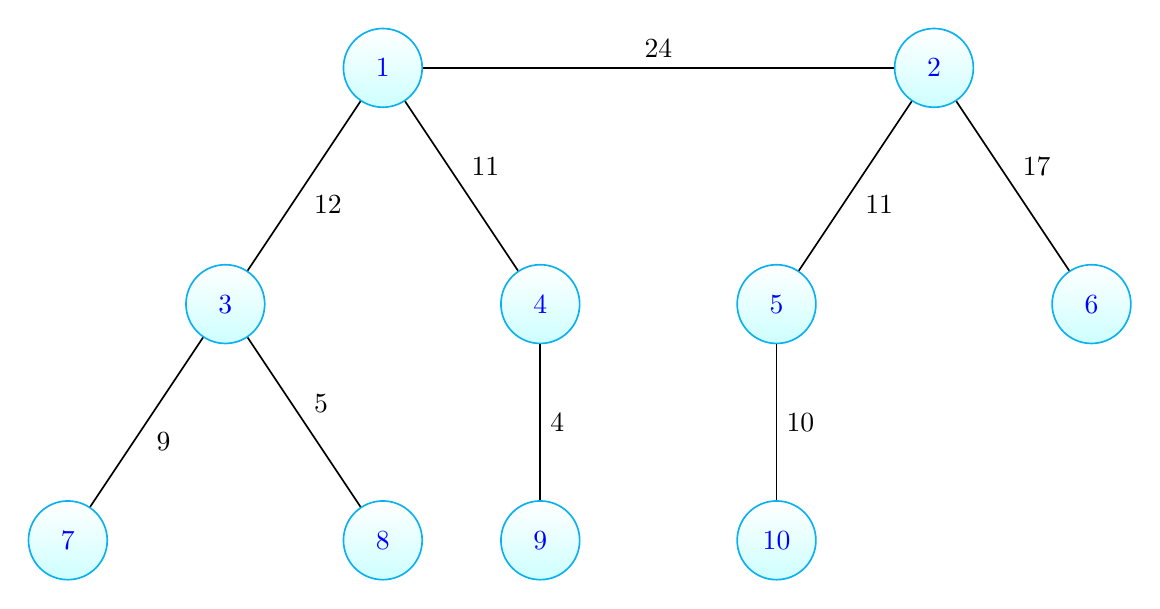
\begin{tikzpicture}[auto ,node distance =2 cm and 5cm ,on grid ,
semithick ,
state/.style ={ circle ,top color =white , bottom color = processblue!20 ,
draw,processblue , text=blue , minimum width =1 cm}]

\node[state] (1) at (-5,0) {1};
\node[state] (2) at (2,0) {2};
\node[state] (3) at (-7,-3) {3};
\node[state] (4) at (-3,-3) {4};
\node[state] (5) at (0,-3) {5};
\node[state] (6) at (4,-3) {6};
\node[state] (7) at (-9,-6) {7};
\node[state] (8) at (-5,-6) {8};
\node[state] (9) at (-3,-6) {9};
\node[state] (10) at (0,-6) {10};

\draw  (1) edge node{24} (2);
\draw  (1) edge node{12} (3);
\draw  (1) edge node{11} (4);
\draw  (3) edge node{9} (7);
\draw  (3) edge node{5} (8);
\draw  (4) edge node{4} (9);

\draw  (2) edge node{11} (5);
\draw  (2) edge node{17} (6);
\draw  (5) edge node{10} (10);
\end{tikzpicture}
\end{center}

\begin{center}
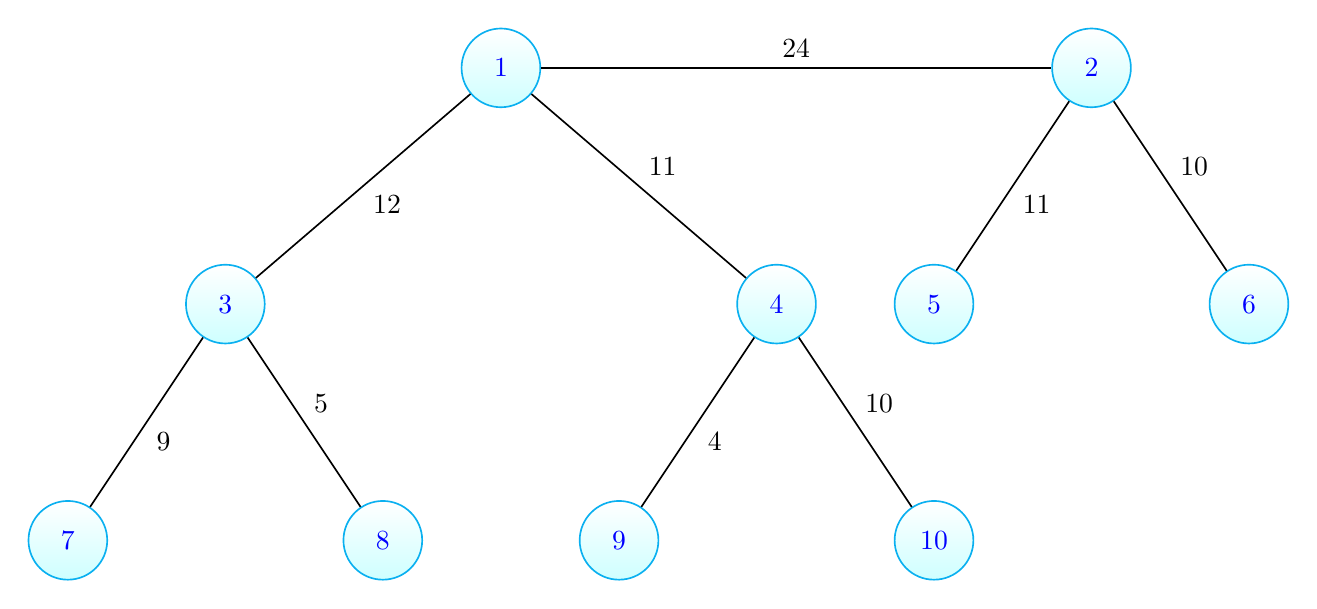
\begin{tikzpicture}[auto ,node distance =2 cm and 5cm ,on grid ,
semithick ,
state/.style ={ circle ,top color =white , bottom color = processblue!20 ,
draw,processblue , text=blue , minimum width =1 cm}]
\node[state] (1) at (-6.5,0) {1};
\node[state] (2) at (1,0) {2};
\node[state] (3) at (-10,-3) {3};
\node[state] (4) at (-3,-3) {4};
\node[state] (5) at (-1,-3) {5};
\node[state] (6) at (3,-3) {6};
\node[state] (7) at (-12,-6) {7};
\node[state] (8) at (-8,-6) {8};
\node[state] (9) at (-5,-6) {9};
\node[state] (10) at (-1,-6) {10};

\draw  (1) edge node{24} (2);
\draw  (1) edge node{12} (3);
\draw  (1) edge node{11} (4);
\draw  (3) edge node{9} (7);
\draw  (3) edge node{5} (8);
\draw  (4) edge node{4} (9);

\draw  (2) edge node{11} (5);
\draw  (2) edge node{10} (6);
\draw  (4) edge node{10} (10);
\end{tikzpicture}
\end{center}


\newpage
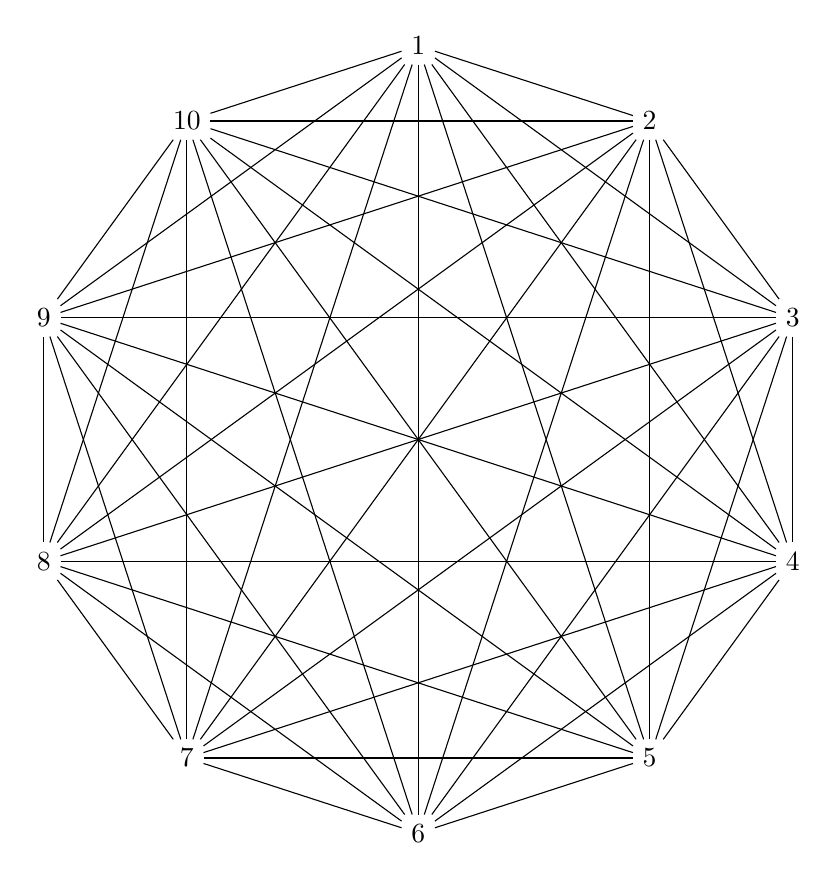
\begin{tikzpicture}
  \graph { subgraph K_n [n=10,clockwise,radius=5cm] };
\end{tikzpicture}

\begin{center}
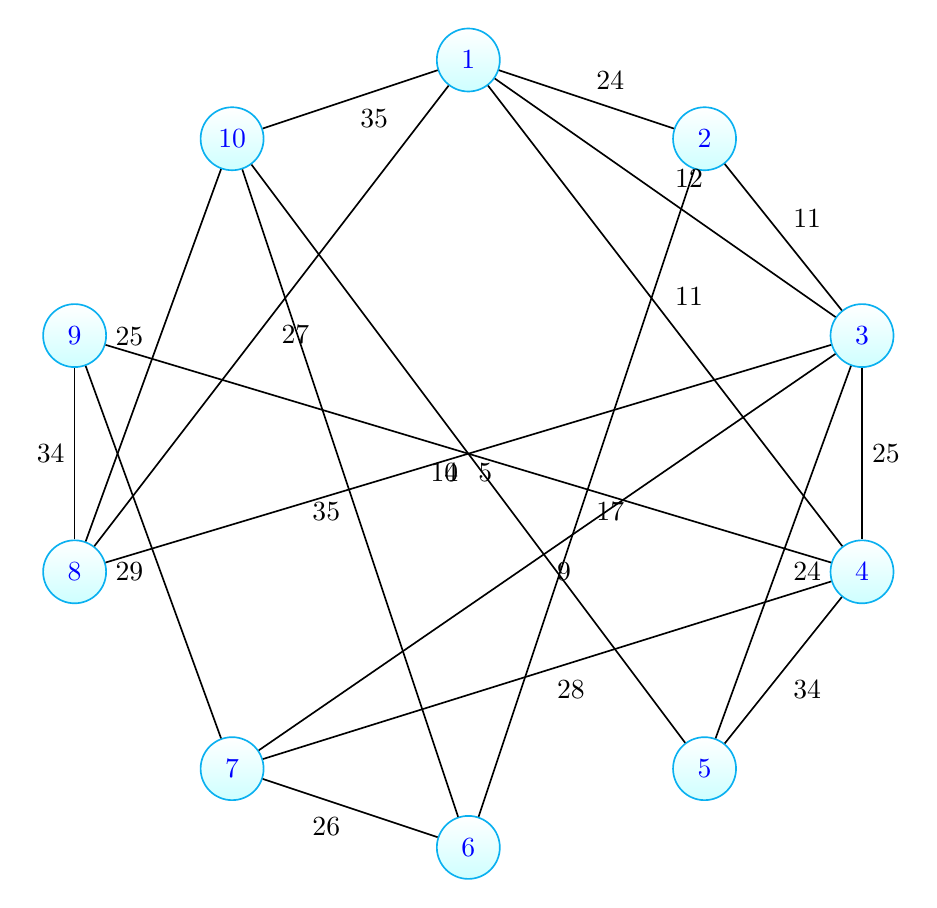
\begin{tikzpicture}[auto ,node distance =2 cm and 5cm ,on grid ,
semithick ,
state/.style ={ circle ,top color =white , bottom color = processblue!20 ,
draw,processblue , text=blue , minimum width =.8 cm}]

\node[state] (1) at (0,5) {1};
\node[state] (6) at (0,-5) {6};

\node[state] (3) at (5,1.5) {3};
\node[state] (9) at (-5,1.5) {9};

\node[state] (4) at (5,-1.5) {4};
\node[state] (8) at (-5,-1.5) {8};

\node[state] (2) at (3,4) {2};
\node[state] (10) at (-3,4) {10};

\node[state] (5) at (3,-4) {5};
\node[state] (7) at (-3,-4) {7};

\draw (1) edge node{24} (2);
\draw (1) edge node{12} (3);
\draw (1) edge node{11} (4);
\draw (1) edge node{35} (10);
\draw (1) edge node{27} (8);



\draw (2) edge node{17} (6);
\draw (2) edge node{11} (3);

\draw (3) edge node{5} (8);
\draw (3) edge node{9} (7);
\draw (3) edge node{25} (4);
\draw (3) edge node{24} (5);

\draw (4) edge node{4} (9);
\draw (4) edge node{34} (5);
\draw (4) edge node{28} (7);

\draw (8) edge node{34} (9);
\draw (8) edge node{25} (10);

\draw (7) edge node{29} (9);

\draw (6) edge node{35} (10);
\draw (6) edge node{26} (7);

\draw (5) edge node{10} (10);



\end{tikzpicture}
\end{center}

\newpage
\begin{center}
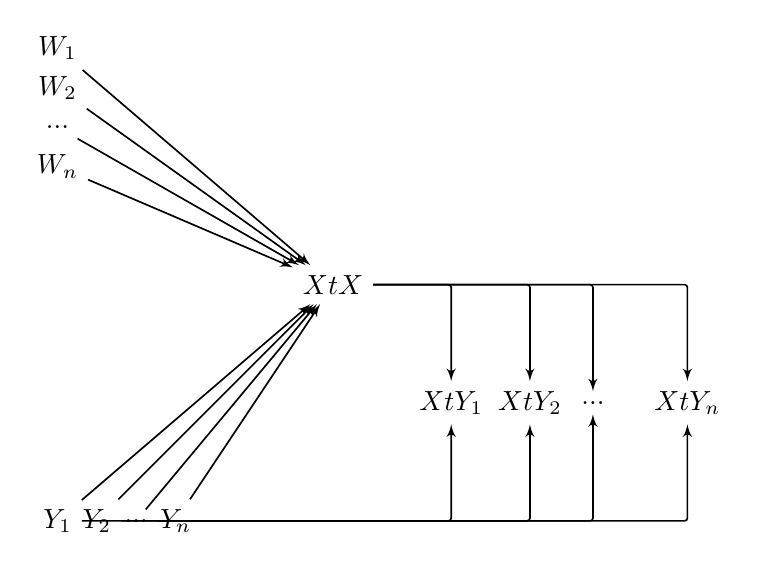
\begin{tikzpicture}[auto ,node distance =2 cm and 5cm ,on grid ,
semithick ,
state/.style ={ },
edge/.style = {->,> = latex'}]


\node (W_1) at (-10,0) {$W_1$};
\node (W_2) at (-10,-.5) {$W_2$};
\node (W_j) at (-10,-1) {$...$};
\node (W_n) at (-10,-1.5) {$W_n$};

\node (Y_1) at (-10,-6) {$Y_1$};
\node (Y_2) at (-9.5,-6) {$Y_2$};
\node (Y_j) at (-9,-6) {$...$};
\node (Y_n) at (-8.5,-6) {$Y_n$};


\node (XtY_1) at (-5,-4.5) {$XtY_1$};
\node (XtY_2) at (-4,-4.5) {$XtY_2$};
\node (XtY_j) at (-3.2,-4.5) {$...$};
\node (XtY_n) at (-2,-4.5) {$XtY_n$};


\node (XtX) at (-6.5,-3) {$XtX$};

\draw[edge]  (W_1) edge  (XtX);
\draw[edge]  (W_2) edge  (XtX);
\draw[edge]  (W_j) edge  (XtX);
\draw[edge]  (W_n) edge  (XtX);

\draw[edge]  (Y_1) edge  (XtX);
\draw[edge]  (Y_2) edge  (XtX);
\draw[edge]  (Y_j) edge  (XtX);
\draw[edge]  (Y_n) edge  (XtX);

\draw[edge,rounded corners=1pt] (XtX) -| (XtY_1);
\draw[edge,rounded corners=1pt] (XtX) -| (XtY_2);
\draw[edge,rounded corners=1pt] (XtX) -| (XtY_j);
\draw[edge,rounded corners=1pt] (XtX) -| (XtY_n);

\draw[edge,rounded corners=1pt] (Y_1) -| (XtY_1);
\draw[edge,rounded corners=1pt] (Y_2) -| (XtY_2);
\draw[edge,rounded corners=1pt] (Y_j) -| (XtY_j);
\draw[edge,rounded corners=1pt] (Y_n) -| (XtY_n);

\end{tikzpicture}
\end{center}


\newpage


\begin{tikzpicture}
\begin{axis}[
    title={Running Time per Iteration Comparison with \textit{sPCA} for $21M$ Sample Count},
    xlabel={Dimensionality (D) of the input matrix ( $\times 10^4$ )},
    ylabel={Running Time Per Iteartion (minutes)},
    xmin=0, xmax=200,
    ymin=0, ymax=80,
    xtick={0,4,8,14,22,30,50,80,100,140,200},
    ytick={0,2,4,6,8,10,20,40,60,80},
    legend pos=north west,
    ymajorgrids=true,
    grid style=dashed,
]

\addplot[
    color=blue,
    ultra thick,
    dotted
    ]
    table {sPCA.dat};
    \addlegendentry{sPCA}
    
\addplot[
    color=black,
    ultra thick
    ]
    table {tall_and_wide.dat};
    \addlegendentry{TallnWide}
    
\end{axis}
\end{tikzpicture}

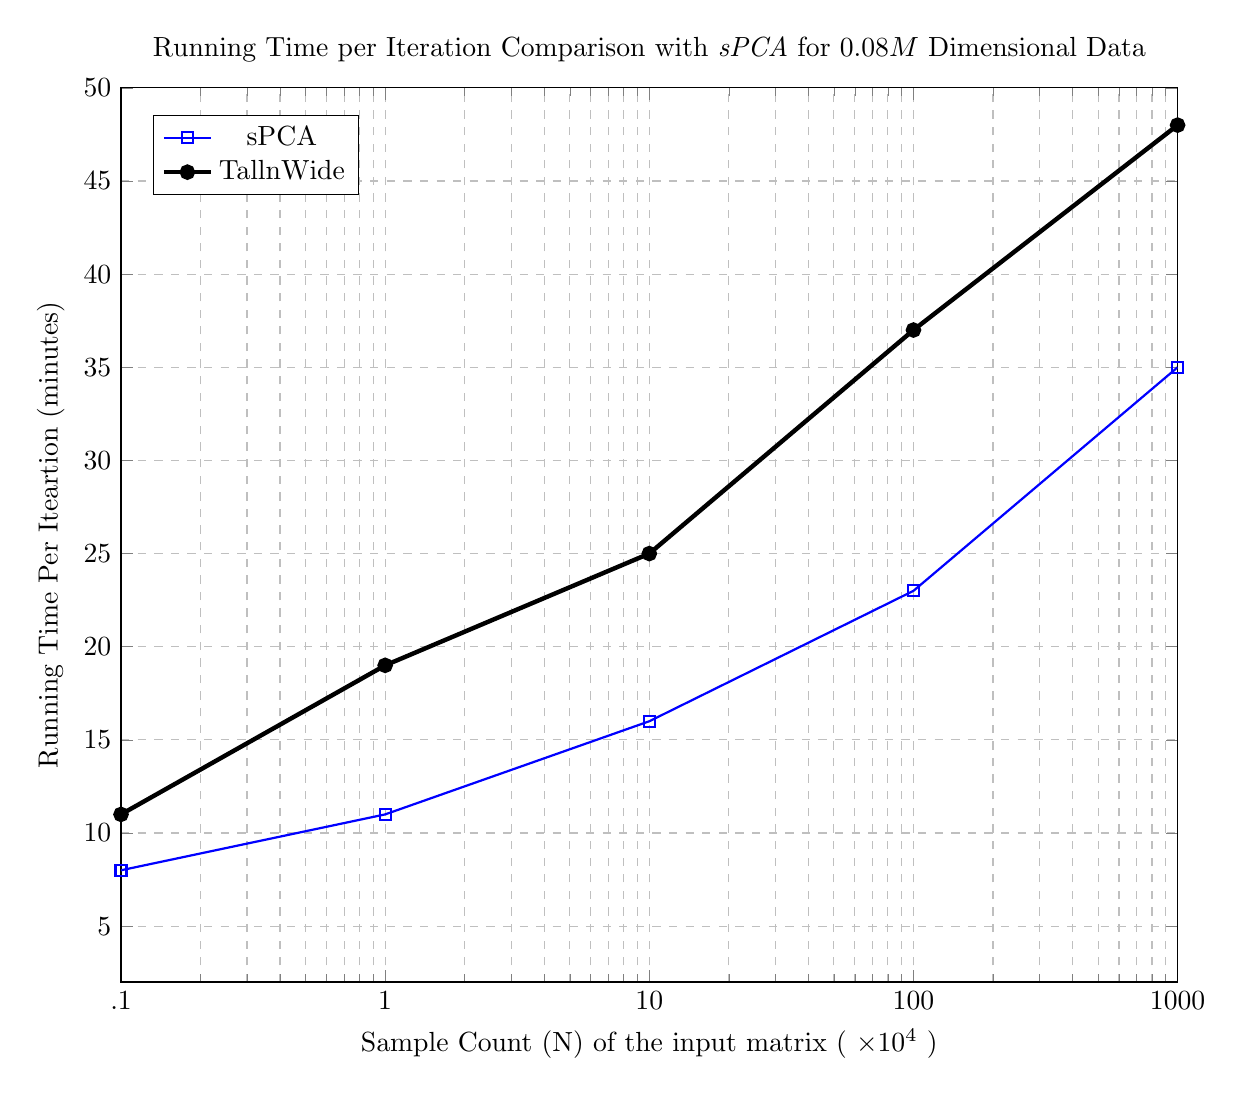
\begin{tikzpicture}
  \begin{axis}[
  	title={Running Time per Iteration Comparison with \textit{sPCA} for $0.08M$ Dimensional Data},
    xlabel={Sample Count (N) of the input matrix ( $\times 10^4$ )},
    ylabel={Running Time Per Iteartion (minutes)},
  	legend pos=north west,
    ymajorgrids=true,
    grid style=dashed,
 	xmode=log,
    xmin=0.1, xmax=1000,
    ymin=2, ymax=50,
    xtick={.1,1,10,100,1000},
    xticklabels={.1,1,10,100,1000},
    grid=both]
    
    \addplot[color=blue,
    mark=square, thick]
    table {
    .1 8
	1 11
	10 16
	100 23
	1000 35
    };
    \addlegendentry{sPCA}
    
    \addplot[mark=*,ultra thick,black]
    table {
    .1 11
	1 19
	10 25
	100 37
	1000 48
    };
    \addlegendentry{TallnWide}
  \end{axis}
\end{tikzpicture}

\end{document}
